\documentclass[pdftex,a4paper,11pt]{article}
\usepackage[utf8]{inputenc}
\usepackage{caption} 
\usepackage[pdftex]{graphicx}
%opening
\title{Project CSSE:\\
       First Deliverable}
\author{Olivier Verhaegen\\	
	overhaeg@vub.ac.be\\
	87116}


\begin{document}

\maketitle


\section{Project Description}

The goal of this project is the implementation of an interpreter of System F$\omega$. System F$\omega$ is an extension of System F, which is itself an extension of 
the Simply Typed Lambda Calculus (STLC). STLC introduces typing to lambda calculus, with a single function operator. 
System F extends STLC by adding support for parametric polymorphism, and System F$\omega$ extends this further with higher-order polymorphism. 
The interpreter will require a Parser, a Type checker and an Evaluator.\\
\noindent
System F$\omega$ will be implemented using the Haskell language, and should therefore be runnable on every system for which an implementation of the Glasgow Haskell Compiler (GHC) exists.
To help with the implementation of the parser we will use the Happy Parser Generator for Haskell.\\
This interpreter was implemented as a three-part project for the course Capita Selecta of Programming Languages. 


\section{Story maps}

The interpreter consists of three distinct parts working together: A Parser, a Type Checker and an Evaluator. Given the nature of the project each part will be implemented 
incrementally to achieve a subset of System F$\omega$. The first subset is the implementation of an interpreter supporting typed artithmetic expression where we will implement the basics of each part. 
The second subset is the implementation of the STLC on top of the first, extending it by adding assignments and function types. The final increment will consist of the implementation of System F$\omega$.\\
Because of this, we consider the first increment of each part as being the most critical and bearing the highest risk, as a problem at this level will cause errors across all the 
expected functionalities of the interpreter. We give a medium risk to the second increment and the lowest risk to the last one. The spliced user story mapping can be seen in Figure 1. 

\begin{center}
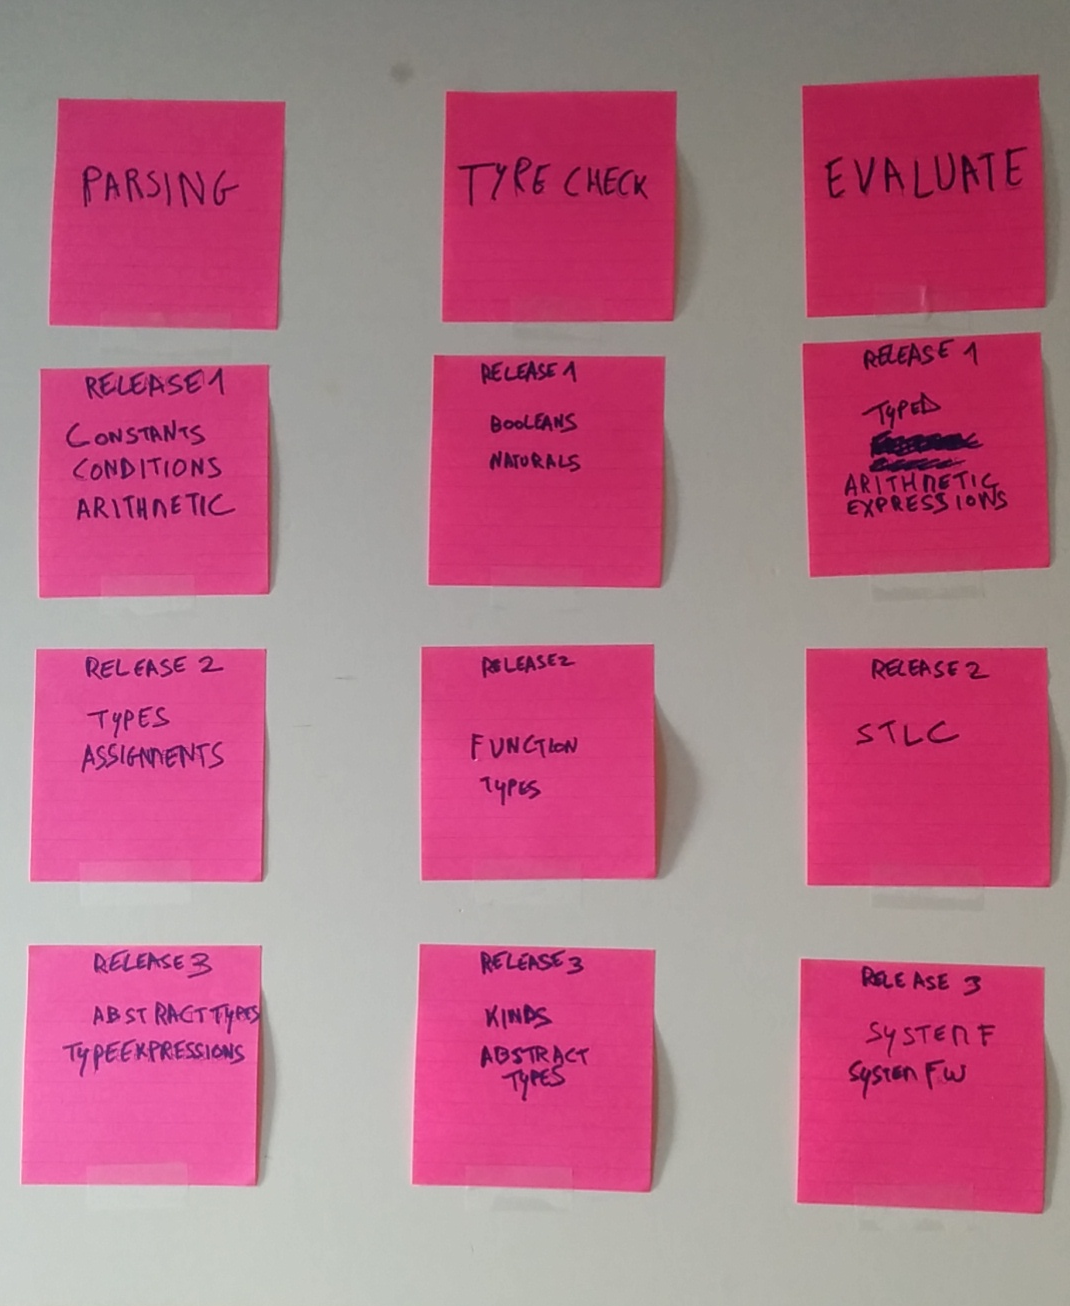
\includegraphics[scale=0.25]{userstorymapping_big.png}
\captionof{figure}{Spliced user story mapping}
\label{registration}
\end{center}

\section{Test Strategy}


\begin{itemize}
  \item Modularity: The interpreter consists of three parts we can consider as units without the need of a refactoring, and we can write unit tests for each of them. We can also write more global tests to test the whole interpreter.
  \item Input/Output: Generating the parsed code that will be used as input and output for various tests is the trickiest part. We could generate it with the Parser but we have to be certain the Parser is correct before using the Parser. 
  We will therefore generate the parser code by hand to be safe.
  \item Test setup: There is some coupling between each part but apart from developing the correct input and output for each test we should not have too much test setup to do.
  \item Coverage: This project does not really have much trivial parts like getters/setters so we aspect a near 100$\%$ coverage, across all user stories. 
\end{itemize}



\section{Planning}
\subsection{Overall Planning}

It is required we spend at least 80 to 100 hours on this project, and we supposedly have three months (14 weeks) to complete this project, which means we should spend an average of 6-7 hours per week on the project. 
We plan on using two milestones, the first one ending on April 20 and the second one at the project deadline. This leaves us 7 weeks for milestone 1 and 7 weeks for milestone 2. 


\paragraph{Milestone 1} \mbox{}\\
Date: March 2 - April 19\\
Time: 40 - 45 hours\\
Objective: Implement the tests related with Release 1 and 2.

\paragraph{Milestone 2} \mbox{}\\
Date: April 20 - June 8\\
Time: 40 - 45 hours\\
Objective: Implement the tests related with Release 3.


\subsection{Detailed planning} 

The next milestone is Milestone 1. We should work on developing tests for releases 1 and 2. We will detail or test strategy for each user story.
\subsubsection{Release 1}

\paragraph{Parser: Constants, Conditions and Arithmetic}
\begin{itemize}
  \item Make a unit test for each symbol that has to be accepted by the Parser.
  \item Make unit tests for symbols the Parser should reject.
  \item Make unit tests to test expressions that should be accepted by the Parser.
\end{itemize}

\paragraph{Type Checker: Booleans and Naturals}
\begin{itemize}
  \item Make unit tests to test if each literal and operation is typechecked correclty
\end{itemize}

\paragraph{Evaluator: Typed Arithmetic Expressions}
\begin{itemize}
  \item Make a unit test to test if each literal and operation is evaluated correclty.
  \item Make unit tests to check that valid typed arithmetic expressions are evaluated correctly.
\end{itemize}

\subsubsection{Release 2}

\paragraph{Parser: Type Assignments and Lambda's}
\begin{itemize}
  \item Make a unit test to test if type assignements are correctly parsed
  \item Make a unit test to check if lambda's are corretly parsed. 
  \item Make multiple unit tests to see if valid STLC expressions are correctly parsed. 
\end{itemize}

\paragraph{Type Checker: Function Types}
\begin{itemize}
  \item Make unit tests to test if functions of various types are typechecked correctly.
\end{itemize}

\paragraph{Evaluator: Simply Typed Lambda Expressions}
\begin{itemize}
  \item Make a unit test to test if type assignements and lambda's are evaluated correclty.
  \item Make unit tests to check that valid STLC expressions are evaluated correctly.
\end{itemize}

\subsubsection{Task Breakdown}
We plan to handle these 12 subtasks in the following way:

\begin{itemize}
  \item Task 1: 1-3 
  \item Task 2: 4-6
  \item Task 3: 7-9
  \item Task 4: 10-12
\end{itemize}

\end{document} 